\chapter{Recurrent Neural Networks}

Limitations of Fully-Connected Neural Networks (FCNNs). They have some inputs and some
output layers, interlieved by some hidden layers.

\begin{figure}[h!]
  \centering
  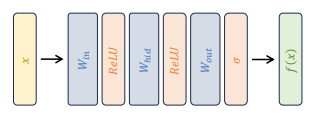
\includegraphics[width=0.3\linewidth]{content/Parts/images/2026-09-28-10-04-11.png}
\end{figure}

This type of models have some architectural constraints

\begin{itemize}
  \item The input/feature is expected to be fixed in size, beacuse each neurons has a specific set of weights
  \item Each input/feature is associated with its set of weights
  \item The output/feature is expected to be fixed in size
\end{itemize}

\subsubsection{The input is expected to be fixed in size}

It is ok when is structured, such as a table. We only manage missing values.
For unstructured and dynamic length data, such as images or text.

\subsubsection{Each input is associated with its set of weights}

If the same pattern occurs in different portions of
the input, the model needs to learn the same
pattern multiple times.


\subsubsection{The output is expected to be fixed in size}

As defined by the number of rows in $W_{out}$. Sometimes, we may want outputs to have 
varying sizes. E.g. In object detection, we want to segment the pixels of an image

\section{Recurrent Neural Networks - RNN}

Type of NN designed to press sequential data. It receave and looks at one element at a time.
And to let the model to remember what it has seen before, we add a hidden state to summarizes
the info seen so far.

\subsubsection{RNN architecture}

The general RNN architecture is charaterized by
two \textbf{inputs} and two \textbf{outputs}:

\begin{itemize}
  \item The first input is the current element of the sequence
  \item The second input is the hidden state from the previous time 
\end{itemize}

\subsubsection{RNN architecture, unfolded}



